\section{Introduction}
\label{s:intro}

Over the last 30 years, Internet congestion control has seen
considerable research interest. Starting with seminal work in the
1980s~\cite{decbit,Jacobson88,chiujain}, the Transmission Control
Protocol (TCP) has adopted a series of end-to-end algorithms to share
network resources among contending
endpoints~\cite{newreno,vegas,cubic,compound}. Another line of work
has explored the use of in-network algorithms running at bottleneck
routers to help perform this function more
efficiently~\cite{Floyd93,ecn,BLUE,AVQ,choke,CoDel,xcp}.

As the Internet grows and evolves, it appears likely that new network
protocols will continue to be developed to accommodate new subnetwork
behaviors and shifting application workloads and goals. Some of these
may be intended for specialized environments---e.g., inside a
centrally-managed datacenter---while some will be for broad use across
the wide-area Internet, or over cellular network paths.

In practice, however, it is challenging to guarantee that a
distributed system's performance in well-characterized testing
scenarios will extend to real networks, which inevitably differ from
those envisioned in development and will continue to evolve over time. This
uncertain generalizability presents an obstacle to any new protocol's
deployment.

In this paper, we formalize the design process for generating
end-to-end congestion-control protocols to quantify: \emph{how easy is
  it to ``learn'' a network protocol to achieve desired goals, given a
  necessarily imperfect model of the networks where it will ultimately
  be deployed?}

Under this umbrella, we examine a series of questions about what
knowledge about the network is important when designing a
congestion-control protocol and what simplifications are acceptable:

\begin{enumerate}

\item \textbf{Knowledge of network parameters.} Is there a tradeoff
  between the performance of a protocol and the breadth of its
  intended operating range of network parameters~\cite{wroclawski}?
  Will a ``one size fits all'' protocol designed for networks spanning
  a thousand-fold range of link rates necessarily perform worse than
  one targeted at a subset of networks whose parameters can be more
  precisely defined in advance?  (\S\ref{s:oprangeperftradeoff})

\item \textbf{Structural knowledge.} How faithfully do protocol
  designers need to understand the topology of the network? What are
  the consequences of designing protocols for a simplified network
  path with a single bottleneck, then running them on networks with
  more-complicated structure?  (\S\ref{ss:topological})

\item \textbf{Knowledge about other endpoints.} In many settings, a
  newly-designed protocol will need to coexist with traffic from
  incumbent protocols. What are the consequences of designing a
  protocol with the knowledge that some endpoints may be running
  incumbent protocols whose traffic needs to be treated fairly
  (e.g.~the new protocol needs to divide a contended link evenly with
  TCP), versus a clean-slate design?  (\S\ref{s:tcpaware})

\item \textbf{Different kinds of breadth.} Will a protocol designed
  for a large range in one kind of network parameter (e.g., the link
  rate) also have broad applicability when other network parameters
  vary, such as the RTT or degree of multiplexing?  Which pairs of
  network parameters are related in this way---such that a protocol's
  breadth in one implies breadth in the other---and which aren't?
  (\S\ref{ss:parameter})

\item \textbf{Knowledge of network signals.} What kinds of congestion
  signals are important for an endpoint to listen to? How much
  information can be extracted from different kinds of feedback, and
  how valuable are different congestion signals toward the protocol's
  ultimate goals?  (\S\ref{s:signals})

\end{enumerate}

\subsection{Tractable attempts at optimal (Tao) protocols}

Each of the above areas of inquiry is about the effect of a protocol
designer's imperfect understanding of the future network that a
decentralized congestion-control protocol will ultimately be run over.

In principle, we would quantify such an effect by evaluating, on the
actual network, the performance of the ``best possible''
congestion-control protocol designed for the imperfect network
\emph{model}, and comparing that with the best-possible protocol for
the actual network itself.

In practice, however, there is no tractable way to calculate the
optimal congestion-control protocol for a given network. Instead,
throughout this study we use the Remy automatic protocol-design
tool~\cite{remy} as a proxy for the optimal solution.

We refer to these automatically-generated congestion-control protocols
as ``tractable attempts at optimal'' (Tao) end-to-end
congestion-control protocols for a given network.  Tao protocols
represent a practically realizable tilt at developing an optimal
protocol for an imperfect model of a real network.

Constructing a Tao for a complex network model requires searching a
huge space, an intensive task even using Remy's search
optimizations. In most cases, the protocol stopped improving within a
CPU-year of processing time (five days on our 80-core machine), though
there were a few cases where improvements continued to occur.

%some cases in our investigation, the protocol continued
%to improve even after the search had consumed more than a CPU-year of
%processing time, or more than five days on an 80-core computer.

\begin{figure}[t!]
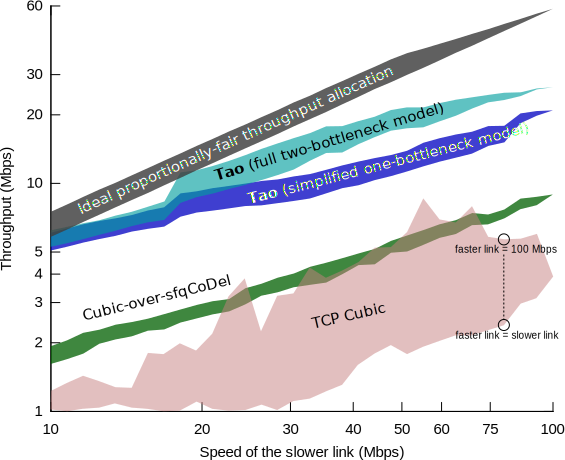
\includegraphics[width=\columnwidth]{figures/plots-10x-new-multilink/multilink-crossing-manual.pdf}
\caption{How well do endpoints need to understand the network around
  them? To assess this, we measure the throughput of four
  congestion-control schemes across a simulated two-hop network path,
  as the rate of each link is swept between 10 and 100~Mbps, with
  75~ms of delay per hop. A tractable attempt at optimal (Tao)
  congestion control for a simplified one-bottleneck model of the
  network performs only a little worse than a protocol designed with
  knowledge of the network's full two-bottleneck structure.}
\label{f:multihop}
\end{figure}

We emphasize that there can be no assurance that the Tao actually
comes close to the optimal congestion-control protocol, except to the
extent that it approaches upper bounds on performance, such as the
ideal fair allocation of network resources. But empirically, such
protocols perform well. Figure~\ref{f:multihop} shows the end-to-end
throughput of connections traversing two bottleneck links for
different protocols, including two Tao protocols. In each experiment,
there were three flows: one that traversed two hops (the measured
connection), a cross-traffic flow that traversed only the first
bottleneck, and another cross-traffic flow that traversed only the
second bottleneck.

%of two Tao protocols, running over a simulated two-hop network path
%and contending with cross traffic that runs over the first or
%second link only.

As the rate of the first and second link are swept between 10 and 100
Mbps, the Tao that was designed for the actual network achieves close
to the ideal proportionally-fair throughput allocation across the two
links. This ideal serves as an upper bound on performance.

A Tao that was designed for a simplified model of the network with
only one hop also performs adequately, but a little worse than the
``full-complexity'' Tao. However, both computer-generated protocols
come closer to the ideal than contemporary protocols in wide use, TCP
Cubic~\cite{cubic}, the default TCP in Linux, and Cubic running over
stochastic fair queueing and CoDel~\cite{CoDel}, an active queue
management (AQM) scheme that runs at both bottlenecks.

%Prior work on computer-generated congestion-control
%protocols~\cite{remy} also found that such algorithms generally
%outperform the breadth of human-designed protocols on the network for
%which they were designed, suggesting they are a fair proxy for the
%optimal congestion-control protocol given a particular network model.

\subsection{Summary of results}

Here are the principal findings of this study:

\vspace{\baselineskip}

\noindent 
\textbf{Modeling a two-bottleneck network as a single bottleneck hurt
  performance only mildly.}  On the two-hop network of
Figure~\ref{f:multihop}, on average we find that a protocol designed
for a simplified, single-bottleneck model of the network
underperformed by {\bf only 17\%} a protocol that was designed with
full knowledge of the network's two-bottleneck structure. The
simplified protocol outperformed TCP Cubic by a factor of $7.2\times$
on average, outperformed Cubic-over-sfqCoDel by $2.75\times$ on
average.

Thus, in this example, full knowledge of the network topology during
the design process was not crucial.

\vspace{\baselineskip}

\noindent 
\textbf{Only weak evidence of a tradeoff between
  operating range and performance.} We created a Tao protocol designed
for a range of networks whose link rates spanned a thousand-fold range
between 1~Mbps and 1000~Mbps, as well as three other protocols that
were more narrowly-targeted at hundred-fold, ten-fold, and two-fold
ranges of link rate (Figure~\ref{fig:breadth}).

The ``thousand-fold'' Tao achieved close to the peak performance of
the ``two-fold'' Tao. Between link rates of 22--44~Mbps, the
``thousand-fold'' Tao achieved \textbf{within 3\% of the throughput}
of the ``two-fold'' protocol that was designed for this exact
range. However, the queueing delay of the ``thousand-fold'' protocol
was \textbf{46\% higher}, suggesting some benefit from more focused
operating conditions. It also takes a lot longer to compute (offline)
a ``thousand-fold'' Tao compared to a two-fold Tao; in run-time
operation, though, the computational cost of the two algorithms is
similar.

Over the full range of 1~Mbps to 1000~Mbps, the ``thousand-fold'' Tao
protocol matched or outperformed TCP Cubic and Cubic-over-sfqCoDel
over the entire range (Figure~\ref{fig:breadth}).

The results suggest that highly optimized protocols may be able to
perform adequately over a broad range of actual networks. Broad
operating range had only a weak effect on peak performance, suggesting
that ``one size fits all'' congestion-control protocols that perform
considerably better than TCP---as well as TCP plus in-network
assistance, in the case of sfqCoDel---may be feasible.


\vspace{\baselineskip}

\noindent \textbf{TCP-awareness hurt performance when TCP
  cross-traffic was absent, but helped dramatically when present.} We
measured the costs and benefits of ``TCP-awareness''---designing a
protocol with the explicit knowledge that it may be competing against
other endpoints running TCP, compared with a ``TCP-naive'' protocol
for a network where the other endpoints only run the same TCP-naive
protocol.

When contending only with other endpoints of the same kind, the
``TCP-naive'' protocol achieved \textbf{55\% less queueing delay} than
the TCP-aware protocol. In other words, ``TCP-awareness'' has a cost
measured in lost performance when TCP cross-traffic is not present
(Figure~\ref{fig:tcpaware}).

But when contending against TCP, the ``TCP-naive'' protocol was
squeezed out by the more-aggressive cross-traffic. By contrast, the
``TCP-aware'' protocol achieved \textbf{36\% more throughput} and
\textbf{37\% less queueing delay} than the ``TCP-naive'' protocol, and
claimed its fair share of the link capacity from TCP.
